\chapter{Introduzione}

\section{Internet:\ una panoramica}

\subsection{Le reti}

Una rete è un'interconnessione di dispositivi in grado di scambiarsi informazioni, quali \emph{sistemi terminali (end system)}, \emph{router}, \emph{switch} e \emph{modem}.\
I sistemi terminali sono chiamati \emph{host}.\
Un host può essere una macchina in genere di proprietà degli utenti e dedicata ad eseguire applicazioni, quale un computer desktop, un portatile, un cellulare o un tablet, oppure un server:\ tipicamente un computer con elevate prestazioni destinato a eseguire programmi che forniscono servizio a diverse applicazioni utente come, per esempio, la posta elettronica o il Web.\
I \emph{router} sono dispositivi che collegano una rete ad altre reti, mentre gli \emph{switch} (commutatori) collegano fra di loro più sistemi terminali a livello locale.\
È possibile che in una rete ci siano anche i modem, che trasformano la codifica dei dati.\
Tutti questi dispositivi vengono collegati utilizzando mezzi trasmissivi cablati o wireless, come cavi o onde radio, genericamente chiamati \emph{link} (collegamenti).

\subsubsection{LAN - \emph{Local Area Network}}

Una LAN (\emph{Local Area Network}), o rete locale, è solitamente una rete privata che collega i computer in un singolo ufficio, un edificio o un comprensorio.\
Qualsiasi sistema terminale in una LAN deve avere un indirizzo che lo identifica univocamente nella rete.\
Un pacchetto inviato da un sistema terminale a un altro contiene entrambi gli indirizzi di mittente e destinatario.

In passato tutti i dispositivi di una rete locale erano collegati mediante un cavo condiviso, o mezzo \emph{broadcast}, per cui il pacchetto inviato da un dispositivo veniva ricevuto da tutti gli altri.\
Il destinatario elaborava il pacchetto, mentre gli altri lo dovevano ignorare.\
Oggi la maggior parte delle LAN utilizza uno switch di interconnessione, al quale ogni dispositivo in rete è direttamente connesso.\
Lo switch è in grado di riconoscere l'indirizzo di destinazione e di inviare quindi il pacchetto al solo destinatario senza inviarlo agli altri dispositivi.\
Lo switch riduce il traffico nella LAN e consente a più coppie di dispositivi di comunicare contemporaneamente fra di loro, posto che non vi siano dispositivi sorgente o destinazione comune.

\subsubsection{WAN - \emph{Wide Area Network}}

Anche una WAN (\emph{Wide Area Network}), o rete geografica, è un'interconnessione di dispositivi in grado di comunicare, ma esistono notevoli differenze rispetto alle LAN.\
Quest'ultime sono solitamente di estensione limitata, mentre una WAN ha un'estensione decisamente superiore, potendo servire una città, una regione, una nazione o addirittura l'intero globo.\
Una LAN interconnette prevalentemente sistemi terminali, mentre una WAN interconnette anche switch, router o modem.\
Una LAN è solitamente di proprietà dell'organizzazione che la utilizza, mentre una WAN è generalmente creata e gestita da un operatore di telecomunicazioni, Internet Service Provider (ISP), che fornisce i suoi servizi alle organizzazioni che ne fanno uso.\
Oggi esistono due tipi di WAN:\ punto-punto e a commutazione (switched).

\paragraph{\emph{WAN punto-punto}}

Una WAN \emph{punto-punto} è una rete che collega due dispositivi di comunicazione tramite un mezzo trasmissivo (cavo o wireless).

\paragraph{\emph{WAN a commutazione}}

Una WAN \emph{a commutazione (switched)} è una rete con più di due punti di terminazione.\
Essa viene utilizzata nelle dorsali dell'odierna rete globale.

\paragraph{\emph{Internetwork}}

Al giorno d'oggi è raro vedere LAN o WAN isolate:\ esse sono in genere connesse fra di loro, formando una \emph{internetwork}, o \emph{internet}.

\subsection{Commutazione (switching)}

Una internet (o internetwork) è data dall'interconnessione di reti, composte da link e dispositivi capaci di scambiarsi informazioni.\
In particolare i sistemi terminali appartenenti alla rete comunicano tra di loro per mezzo di dispositivi come switch e router che si trovano nel percorso (o rotta) tra il sistema sorgente e destinazione.\
In base al metodo adottato per determinare il percorso tra due sistemi terminali in comunicazione si possono distinguere due tipi di reti:\ a commutazione di circuito e a commutazione di pacchetto.

\paragraph{\emph{Reti a commutazione di circuito}}

In una rete a commutazione di circuito (\emph{circuit-switched network}) tra due dispositivi è sempre disponibile un collegamento dedicato, chiamato circuito; lo switch che collega i due dispositivi può solo attivarlo o disattivarlo.\
Sul percorso vengono dedicate risorse alla comunicazione e sono garantite per tutta la sua durata.

\vspace{12pt}
\noindent Svantaggi
\begin{itemize}
    \item necessaria una fase di instaurazione (\emph{setup}) della comunicazione;
    \item le risorse rimangono inattive se non utilizzate (non c'è condivisione).
\end{itemize}
Vantaggi
\begin{itemize}
    \item performance (garantita)
\end{itemize}

\paragraph{\emph{Reti a commutazione di pacchetto}}

In una rete di computer la comunicazione fra i due lati viene effettuata trasmettendo blocchi di dati chiamati \emph{pacchetti}.\
Invece di avere una comunicazione continua, i due computer comunicano scambiandosi pacchetti di dati.\
Gli switch sono in grado di memorizzare i pacchetti, oltre che inoltrarli, essendo i pacchetti entità indipendenti che possono essere memorizzate e inviate successivamente.\
Mentre la commutazione di circuito prealloca l'utilizzo del collegamento trasmissivo con collegamenti garantiti, nella commutazione di pacchetto, pacchetto dopo pacchetto la capacità trasmissiva dei collegamenti sarà condivisa solo tra gli utenti che devono trasmettere sul collegamento.\
La sequenza dei pacchetti non segue uno schema prefissato, la condivisione di risorse avviene su richiesta (detta anche multiplexing statistico delle risorse).

\vspace{12pt}
\noindent Vantaggi
\begin{itemize}
    \item le risorse vengono usate \emph{a seconda delle necessità}
\end{itemize}
Svantaggi
\begin{itemize}
    \item Contesa per le risorse
          \begin{itemize}
              \item la richiesta di risorse può eccedere il quantitativo disponibile;
              \item congestione:\ accodamento dei pacchetti, attesa per l'utilizzo del collegamento.
          \end{itemize}
    \item Trasmissione \emph{store-and-forward}
          \begin{itemize}
              \item il commutatore (es.\ router) deve ricevere l'intero pacchetto prima di poter cominciare a trasmettere sul collegamento in uscita:\ ritardo di store and forward
              \item attesa dei pacchetti in code di output (buffer):\ ritardo di coda
              \item i buffer hanno dimensione finita:\ perdita di pacchetti
          \end{itemize}
\end{itemize}

\subsection{Internet}

Una internet (con \emph{i minuscola}) è costituita da due o più reti interconnesse.\
L'internet più famosa è chiamata Internet (\emph{I maiuscola}) ed è composta da migliaia di reti interconnesse.\
Ogni rete connessa a Internet deve usare l'Internet Protocol (IP) e rispettare certe convenzioni su nomi e indirizzi.\
Nuove reti si aggiungono facilmente.\
Le reti degli host sono connesse a Internet attraverso una gerarchia di fornitori di servizi Internet (Internet Service Provider).\
Al livello più alto ci sono le dorsali, reti particolarmente estese di proprietà di qualche compagnia telefonica.\
Queste reti dorsali sono interconnesse tramite sistemi di comunicazione notevolmente complessi, chiamati \emph{peering point}; si possono anche definire degli \emph{Internet eXchange Point} (IXP):\ punto di incontro (può essere gestito da un'azienda terza) per il peering tra due o più ISP.\
Al secondo livello vi sono reti più piccole, chiamate reti dei provider, che utilizzano a pagamento i servizi delle dorsali.\
Le reti dei provider sono connesse alle dorsali e a volte ad altre reti di provider.\
Le reti private sono reti ai confini di Internet che utilizzano i servizi a pagamento forniti dalle reti dei provider.\
Le dorsali sono spesso chiamate ISP internazionali, le reti dei provider ISP nazionali o regionali.

\paragraph{\emph{Vista dei ``servizi''}}

Infrastruttura che fornisce servizi di comunicazione alle applicazioni:\
\begin{itemize}
    \item WWW, email, giochi, e-commerce, database, controllo remoto, voice over IP, ecc.
    \item applicazioni distribuite che coinvolgono più host
\end{itemize}
Si distinguono due tipi di servizi fondamentali
\begin{itemize}
    \item senza connessione (\emph{connectionless}):\ senza garanzia di consegna;
    \item orientati alla connessione (\emph{connection-oriented}):\ garantiti in integrità, completezza e ordine.
\end{itemize}

\paragraph{\emph{Vista ``delle entità software''}}

\begin{itemize}
    \item \textbf{Applicazioni}:\ elaborano e si scambiano le informazioni
    \item \textbf{Protocolli}:\ regolamentano la trasmissione e la ricezione dei messaggi (es.\ TCP, IP, HTTP, FTP, PPP)
    \item \textbf{Interfacce}:\ definite in seguito, sono le ``membrane'' che separano gli strati della pila protocollare
\end{itemize}
\textbf{\emph{Gli standard Internet e del Web}}
\begin{itemize}
    \item \textbf{Internet Engineering Task Force (IETF)}:\ l'organismo che studia e sviluppa i protocolli in uso su Internet.\ Si basa su gruppi di lavoro a cui chiunque può partecipare.
    \item \textbf{Internet Corporation for Assigned Names and Numbers (IC\-ANN)}:\ coordina il sistema dei nomi di dominio (DNS), assegna i gruppi di indirizzi di rete, identificativi di protocollo e ha funzioni di controllo (blando) dello sviluppo di Internet
    \item \textbf{World Wide Web Consortium (W3C)}:\ comunità internazionale che sviluppa standard aperti per favorire lo sviluppo del Web (es.\ HTML, XML, Semantic Web, ecc.)
\end{itemize}

\subsection{L'accesso a Internet}

Internet è una internetwork che consente a qualsiasi utente di farne parte.\
L'utente, tuttavia, deve essere fisicamente collegato a un ISP, solitamente mediante una WAN punto-punto.\
Il collegamento che connette l'utente al primo router di Internet è detto rete di accesso.\
Le reti di accesso sono di varia tipologia:\
\begin{itemize}
    \item accesso via rete telefonica
          \begin{itemize}
              \item servizio dial-up
              \item Digital Subscriber Line (DSL)
              \item tecnologie per accesso in fibra ottica
          \end{itemize}
    \item accesso tramite reti wireless
          \begin{itemize}
              \item 3G, 4G, 5G
          \end{itemize}
    \item collegamento diretto (es.\ collegamenti WAN dedicati ad alta velocità)
\end{itemize}

\subsection{Metriche di riferimento}

Un argomento di cui si parla spesso nell'ambito delle reti è la velocità della rete o di un collegamento, ovvero quanto velocemente si riesce a trasmettere e ricevere dati.\
In realtà, il concetto di velocità è molto ampio e coinvolge vari fattori che influiscono sulle prestazioni (\emph{performance}) di una rete.

\subsubsection{\emph{Ampiezza di banda e bit rate}}

Con il termine ampiezza di banda si indicano due concetti leggermente diversi ma strettamente legati.\
Al livello di caratterizzazione di un canale o di un sistema trasmissivo, l'ampiezza di banda (\emph{bandwidth}), o banda, è una quantità che si misura in hertz e rappresenta la larghezza dell'intervallo di frequenze utilizzato dal sistema trasmissivo, ovvero l'intervallo di frequenze che un mezzo fisico consente di trasmettere senza danneggiare il segnale in maniera irrecuperabile.\
In generale, maggiore è l'ampiezza di banda, maggiore è la quantità di informazione che può essere veicolata attraverso il mezzo trasmissivo.

Quando viene espressa in bit al secondo (bps), la banda rappresenta invece il \emph{bit} o \emph{trasmission rate} (velocità di trasmissione), per brevità \emph{rate}, ovvero la quantità di bit al secondo che un certo link garantisce di trasmettere.\
I due concetti sono legati ma non coincidenti, in quanto il bit rate di un link dipende sia dalla banda (in hertz) che dalla specifica tecnica di trasmissione, o formato di modulazione digitale utilizzato.\
In generale, il bit rate è proporzionale alla banda in hertz.\
Infine, per banda di un tipo di rete, si intende il bit rate garantito (nominalmente) dai suoi link.

\subsubsection{\emph{Throughput}}

Il throughput indica quanto velocemente riusciamo effettivamente a inviare i dati tramite una rete.\
Sebbene a prima vista il rate e il throughput sembrino la stessa cosa, in realtà non lo sono.\
Un link può avere un rate di \emph{B} bps, ma possiamo inviare solo \emph{T} bps tramite quel link, con \emph{T} sempre inferiore a \emph{B}.\
In altre parole, il rate è una misura della potenziale velocità di un link; il throughput è una misura dell'effettiva velocità di un link (quanto velocemente riusciamo a inviare i dati in realtà).\
È importante notare che il throughput è definito come il numero dei bit che passano attraverso un punto della rete in un secondo.\
In un percorso da una sorgente a una destinazione un pacchetto può passare attraverso numerosi link, ognuno con un throughput diverso:\ il throughput medio è determinato dal collo di bottiglia.\
In generale in un percorso con \emph{n} link in serie abbiamo
\begin{center}
    $Throughput = \min\{T_1, T_2, \dots, T_n\}$.
\end{center}
Si noti che il throughput dipende non solo dalla velocità di trasmissione del collegamento ma anche dalla quantità di dati (flussi di traffico aggiuntivi rispetto a quello di interesse), \textbf{effetti dei protocolli}, ecc.

\subsubsection{\emph{Latenza (ritardo)}}

La latenza, o ritardo (delay), definisce quanto tempo serve affinché un intero messaggio arrivi completamente a destinazione dal momento in cui il primo bit parte dalla sorgente.\
I ritardi si possono dividere in quattro tipi:\ \emph{ritardo di trasmissione}, \emph{ritardo di propagazione}, \emph{ritardo di elaborazione} e \emph{ritardo di accodamento}.\
La latenza, o ritardo totale, deriva dalla seguente formula:\
\begin{center}
    \textbf{Latenza = ritardo di propagazione + ritardo di trasmissione + ritardo di accodamento + ritardo di elaborazione}
\end{center}
\begin{itemize}
    \item \textbf{Ritardo di propagazione}:\ tempo che serve a un bit per viaggiare da un punto A a un punto B sul mezzo trasmissivo.\ Dipende dalla distanza (valori tipici da pochi microsecondi a centinaia di millesecondi)
          \begin{center}
              $Ritardo_{pr} = distanza/velocit\grave{a}_{propagazione}$
          \end{center}
    \item \textbf{Ritardo di trasmissione}:\ tempo necessario per immettere un pacchetto sulla linea
          \begin{center}
              $Ritardo_{tr} = lunghezza del pacchetto/rate_{trasmissione}$
          \end{center}
    \item \textbf{Ritardo di accodamento}:\ tempo in cui il pacchetto attende nella coda del router (dipende dalla congestione)
    \item \textbf{Ritardo di elaborazione}:\ tempo per l'elaborazione al nodo intermedio (in genere pochi microsecondi, o anche meno)
\end{itemize}

\subsubsection{\emph{Perdita di pacchetti}}

Un'altra questione che influisce gravemente sulle prestazioni della comunicazione è il numero di pacchetti persi durante la trasmissione.\
Quando un router riceve un pacchetto mentre ne sta elaborando un altro, il pacchetto ricevuto deve essere memorizzato nel buffer di input in attesa del suo turno.\
Un router tuttavia ha un buffer di input di dimensioni limitate.\
Può arrivare il momento in cui il buffer è pieno e il pacchetto successivo deve essere saltato.\
L'effetto della perdita del pacchetto è che deve essere inviato nuovamente, il che a sua volta può creare un'eccedenza di dati e causare la perdita di altri pacchetti.

\subsubsection{\emph{Ritardo end-to-end}}

Ipotizzando che ci siano \emph{N-1} router tra origine e destinazione e che siano trascurabili i ritardi di congestione, che il ritardo di elaborazione ai router e al nodo mittente sia Ritardo\textsubscript{el}, il ritardo di trasmissione sia Ritardo\textsubscript{tr} e il ritardo di propagazione su ciascun collegamento valga Ritardo\textsubscript{pr}
\begin{center}
    $Ritardo_{nodo} = Ritardo_{el} + Ritardo_{tr} + Ritardo_{pr} $\\
    $Ritardo_{end-to-end} = N\cdot Ritardo_{nodo}$
\end{center}
Nel caso generale di ritardi eterogenei
\begin{center}
    $Ritardo_{end-to-end} = Ritardo_{nodo1} + Ritardo_{nodo2} + \dots + Ritardo_{nodoN}$
\end{center}

\subsubsection{\emph{Prodotto rate-ritardo}}

Il rate e il ritardo sono due metriche delle prestazioni di un link.\
Tuttavia, ciò che è realmente importante nella comunicazione dei dati è il loro prodotto:\ numero massimo di bit che il link può contenere.

\section{L'organizzazione dei protocolli in livelli}

Un termine che si utilizza frequentemente quando si parla di Internet è protocollo.\
Un protocollo definisce le regole che il mittente e il destinatario, così come tutti i sistemi intermedi coinvolti, devono rispettare per essere in grado di comunicare.\
In situazioni particolarmente semplici potrebbe essere sufficiente un solo protocollo, in situazioni più complesse potrebbe essere opportuno suddividere i compiti fra più livelli (\emph{layer}), nel qual caso è richiesto un protocollo per ciascun livello:\ si parla dunque di \emph{layering di protocolli}, o di organizzazione (o strutturazione) dei protocolli in livelli.

\subsection{Stratificazione}

Scomposizione dei sistemi complessi:\
\begin{itemize}
    \item la struttura esplicita permette l'identificazione delle relazioni tra gli elementi di un sistema complesso
          \begin{itemize}
              \item \emph{modello di riferimento stratificato}
              \item \emph{suddivisione di funzioni e attori}
          \end{itemize}
    \item la modularizzazione facilita la manutenzione e l'aggiornamento del sistema
          \begin{itemize}
              \item un modulo (o più precisamente livello/strato) svolge un insieme delimitato di compiti e nel sistema appare come una black box (input/output)
              \item ciascun livello offre servizi allo strato superiore implementando azioni all'interno del livello stesso e utilizzando i servizi del livello inferiore
          \end{itemize}
    \item separazione tra servizi offerti (interfaccia) e implementazione:\ il cambiamento dell'implementazione di un servizio in un livello è sostanzialmente trasparente per il resto del sistema.
\end{itemize}
\textbf{\emph{Principi base della stratificazione}}
\begin{itemize}
    \item \textbf{\emph{Separation of Concern}}:\ separazione degli interessi e delle responsabilità, fare ciò che compete, delegando ad altri tutto ciò che è delegabile
    \item \textbf{\emph{Information Hiding}}:\ nascondere tutte le informazioni che non sono indispensabili affinché il committente possa compiutamente definire l'operazione
\end{itemize}

\subsubsection{In sintesi}

\begin{itemize}
    \item \textbf{Modello stratificato}
          \begin{itemize}
              \item costituito da sistemi di consumatori/produttori
              \item sistemi organizzati in strati funzionali (livelli)
              \item ogni strato fornisce servizi allo strato superiore e usa i servizi di quello inferiore
              \item ogni stato scambia informazioni direttamente solo con gli strati adiacenti
              \item in ogni comunicazione i due strati omologhi svolgono funzioni reciproche
              \item esistono sistemi (intermedi) che implementano solo alcune funzioni
          \end{itemize}
    \item \textbf{Requisiti}
          \begin{itemize}
              \item efficiente:\ minimizzare lo sforzo globale
              \item efficace:\ massimizzare i risultati
          \end{itemize}
          \pagebreak
    \item \textbf{Vantaggi}
          \begin{itemize}
              \item scompone il problema in sottoproblemi più semplici da trattare:\ il singolo strato è più semplice del sistema nel suo complesso
                    \begin{itemize}
                        \item semplificazione della progettazione, implementazione e manutenzione del software
                    \end{itemize}
              \item rende i vari livelli indipendenti:\ posso modificare l'implementazione di uno strato senza dover cambiare gli altri strati (adiacenti e non), a patto che l'interfaccia non cambi
                    \begin{itemize}
                        \item i servizi forniti dagli strati inferiori possono essere usati da più entità negli strati adiacenti superiori
                    \end{itemize}
              \item definendo solamente servizi e interfacce, i livelli diversi possono essere sviluppati da soggetti diversi
          \end{itemize}
\end{itemize}

\subsubsection{Criteri di stratificazione}

\begin{itemize}
    \item Ogni livello logico di astrazione è realizzato in un apposito strato:\ un livello viene creato quando si rende necessario un diverso grado di astrazione.
    \item Ogni strato svolge una sola e ben definita funzione
    \item Il flusso dati attraverso le interfacce di ogni strato deve essere minimizzato
    \item Il numero degli strati deve essere minimizzato, compatibilmente con la loro complessità:\ numero sufficientemente alto per garantire che nessun livello sia troppo complesso e contenga troppe funzioni, ma anche sufficientemente basso per non rendere troppo onerosa l'integrazione e l'architettura poco flessibile
\end{itemize}

\subsection{OSI RM - \emph{Open System Interconnection}}

Le prime reti di calcolatori nascono come \emph{sistemi chiusi}:\ rete specializzata per specifici servizi e nella quale tutti i componenti sono dello stesso costruttore.\
Tuttavia, tali sistemi portano a problemi di interoperabilità poiché gli apparati non riescono ad interpretare i segnali degli altri in altre reti (parlano linguaggi diversi) e di conseguenza i programmi applicativi non riescono ad operare in ambiente distribuito.\
Da qui l'esigenza di realizzare dei \emph{sistemi aperti}, ovvero dei sistemi in cui si stabiliscono delle regole comuni; vengono definiti degli standard con l'obiettivo di realizzare reti di calcolatori che potessero colloquiare con reti e dispositivi di altri fornitori.

Un sistema aperto (\emph{open system}) è un sistema che implementa protocolli aperti:\
\begin{itemize}
    \item i dettagli dei protocolli sono disponibili pubblicamente;
    \item i cambiamenti sono gestiti da un'organizzazione la cui partecipazione è aperta al pubblico.
\end{itemize}
L'\textbf{\emph{International Organization for Standards} (ISO)} ha specificato uno standard per l'interconnessione di sistemi aperti:\ modello di riferimento \emph{Open System Interconnection} (OSI).\
OSI ha molto influenzato il modo di pensare ai protocolli stratificati.

\subsubsection{Modello ISO/OSI}

Il modello ISO/OSI prevede di dividere le funzionalità del protocollo di telecomunicazione in strati, o layers, ognuno dei quali svolge una parte piccola e indipendente dalle altre allo scopo di permettere una realizzazione o revisione delle singole fuzionalità senza dover toccare le altre o anche di permettere una compatibilità a livelli diversi tra diverse implementazioni.\
La comunicazione tra i vari livelli è assicurata da chiamate standard; ogni livello è tenuto a rispondere in maniera corretta alle chiamate che gli competono e che verranno generate dai due livelli ad esso adiacenti (superiore e inferiore).\
La modalità con cui le funzioni competenti ad un livello vengono svolte non è visibile dall'esterno che ne è così svincolato.

\paragraph{Modello a strati}

\begin{itemize}
    \item Uno strato fornisce servizi allo strato superiore e riceve servizi dallo strato inferiore
    \item Lo strato \emph{n-esimo} di una entità comunica con lo strato \emph{n-esimo} di un'altra entità secondo un protocollo assegnato
    \item La comunicazione tra due strati avviene attraverso un'interfaccia
\end{itemize}

\paragraph{Definizioni}

\begin{itemize}
    \item \textbf{Strato}:\ modulo interamente definito attraverso i servizi, protocolli e le interfacce che lo caratterizzano (spesso indicato come livello)
    \item \textbf{Servizio}:\ insieme di primitive (operazioni) che uno strato fornisce ad uno strato soprastante
    \item \textbf{Interfaccia}:\ insieme di regole che governano il formato e il significato delle unità di dati (es.\ messaggi, segmenti, o pacchetti) che vengono scambiati tra due strati adiacenti della stessa entità
    \item \textbf{Protocollo}:\ insieme di regole che
          \begin{itemize}
              \item permettono a due entità omologhe uno scambio efficace e efficiente delle informazioni
              \item definiscono il formato e l'ordine dei messaggi inviati e ricevuti tra entità omologhe della rete e le azioni che vengono fatte per la trasmissione e ricezione dei messaggi.
          \end{itemize}
\end{itemize}

\subsubsection{Pila di Protocolli - \emph{Protocol Stack}}

Strati di supporto alla rete e infrastruttura trasmissiva:\ trasmissione dei dati (realizzazione software e hardware)
\begin{itemize}
    \item Protocollo di livello 1 \textbf{fisico}:\ trasmette un flusso di bit
    \item Protocollo di livello 2 \textbf{datalink}:\ consegna trame sul link
    \item Protocollo di livello 3 \textbf{rete}:\ instradamento del traffico
    \item Protocollo di livello 4 \textbf{trasporto}:\ trasferimento dati tra host
\end{itemize}
Strati di supporto all'elaborazione e interazione con utente (realizzazione software)
\begin{itemize}
    \item  Protocollo di livello 5 \textbf{sessione}:\ controllo del dialogo
    \item  Protocollo di livello 6 \textbf{presentazione}:\ unificazione dati
    \item  Protocollo di livello 7 \textbf{applicazione}:\ elaborazione dati
\end{itemize}
Inoltre, è possibile avere dei nodi intermedi:\ nello schema teorico di principio i primi 4 livelli superiori del modello ISO/OSI si riferiscono al dialogo \emph{end-to-end}, cioè fra host terminali, mentre dal livello \emph{rete} in giù si gestisce il trasferimento dati tra nodi intermedi.

Per quanto riguarda il livello \emph{trasporto} abbiamo due modalità di servizio fondamentali:\
\begin{itemize}
    \item \emph{connection-oriented}, nella quale c'è un'associazione logica tra due o più sistemi e, anche se siamo in una rete di commutazione di pacchetto, si riesce a costruire l'astrazione di connessione (instaurazione della connessione, trasferimento dei dati, chiusura della connessione);
    \item \emph{connection-less}, dove i dati vengono trasferiti end-to-end ma senza stabilire una connessione.
\end{itemize}

\subsubsection{Flusso dell'informazione}

Per la rete, l'informazione ha origine al livello \emph{applicazione} e discende i vari livelli fino alla trasmissione sul canale \emph{fisico}.\
Ogni livello aggiunge all'informazione del livello superiore una propria sezione informativa, o più di una (\textbf{\emph{incapsulamento}}):\ header che contiene informazioni riguardanti esclusivamente quel livello.\
Per i dati ricevuti si segue il cammino inverso:\ processo inverso.\
La definizione di \emph{incapsulamento} è tale da garantire la possibilità di estrarre i dati precedentemente incapsulati.

Incapsulamento
\begin{itemize}
    \item \textbf{Header}:\ qualificazione del pacchetto dati per questo livello;
    \item \textbf{Data}:\ payload proveniente dal livello superiore
    \item \textbf{Trailer}:\ generalmente usato in funzione di trattamento dell'errore (rivelazione, correzione)
\end{itemize}

\subsection{Lo stack protocollare TCP/IP}

TCP/IP è una famiglia di protocolli attualmente utilizzata in Internet.\
Si tratta di una gerarchia di protocolli, costituita da moduli interagenti, ciascuno dei quali fornisce funzionalità speficiche.\
Il termine gerarchia significa che ciascun protocollo di livello superiore è supportato dai servizi forniti dai protocolli di livello inferiore.\
Tale organizzazione dei protocolli viene chiamata \emph{pila} o \emph{stack protocollare TCP/IP}.\
Definita in origine in termini di quattro livelli software soprastanti a un livello hardware, la pila TCP/IP è oggi intesa come composta di 5 livelli:\
\begin{enumerate}
    \item \emph{fisico}
    \item \emph{link}
    \item \emph{rete}
    \item \emph{trasporto}
    \item \emph{applicazione}
\end{enumerate}
Il compito dei livelli \emph{applicazione}, \emph{trasporto} e \emph{rete} è di tipo end-to-end, ovvero fra i due host terminali coinvolti nella comunicazione.\
Invece il compito dei livelli di \emph{collegamento} e \emph{fisico} è \emph{hop-to-hop}, dove un \emph{hop} è un host o un router.\
In altre parole il dominio dei compiti dei tre livelli superiori è la internet, mentre il dominio dei compiti dei due livelli inferiori è il link.

\subsubsection{\emph{Livello applicazione}}

La comunicazione al livello applicazione avviene tra due \emph{processi} (due programmi eseguiti a questo livello).\
Per comunicare, un processo invia una richiesta all'altro processo e ne riceve una risposta.\
Questo livello in Internet prevede numerosi protocolli predefiniti:\ HTTP, SMTP, FTP, \dots

\subsubsection{\emph{Livello di trasporto}}

Il livello di trasporto nell'host sorgente riceve il messaggio dal livello applicazione, lo incapsula in un pacchetto di livello di trasporto (chiamato \emph{segmento}) e lo invia, tramite la connessione logica (virtuale), al livello di trasporto dell'host destinatario.\
Esistono più protocolli a livello di trasporto:\ TCP, UDP.

\subsubsection{\emph{Livello di rete}}

Il livello di rete (network) è responsabile della comunicazione host-to-host e dell'instradamento e inoltro dei pacchetti attraverso i possibili percorsi.\
I protocolli di questo livello sono:\ IP, ICMP.

\subsubsection{\emph{Livello di link}}

Il livello di collegamento (\emph{data-link}) si occupa del trasferimento dati in frame attraverso il collegamento tra elementi di rete vicini.

\subsubsection{\emph{Livello fisico}}

Il livello fisico si occupa di trasferire i singoli bit di un frame attraverso il link.

\subsubsection{Incapsulamento}

A livello applicazione i dati da scambiare vengono chiamati \emph{messaggi}.\
Un messaggio solitamente non contiene alcuna \emph{intestazione} (\emph{header}) o \emph{trailer}.\
Il messaggio viene passato al livello trasporto.

Il livello trasporto considera il messaggio ricevuto come \emph{payload}, ovvero come carico dati, che deve trasportare e gli aggiunge il suo header; il risultato dell'incapsulamento è un \emph{segmento}.

Il livello di rete considera il pacchetto di livello trasporto passatogli come proprio carico dati e gli aggiunge un'intestazione, il risultato è un pacchetto di livello di rete, chiamato \emph{datagramma}.

Il livello di collegamento considera il pacchetto di livello di rete come payload e gli aggiunge la propria intestazione, il risultato è un pacchetto di livello di collegamento, chiamato \emph{frame}.

\begin{figure}[H]
    \centering
    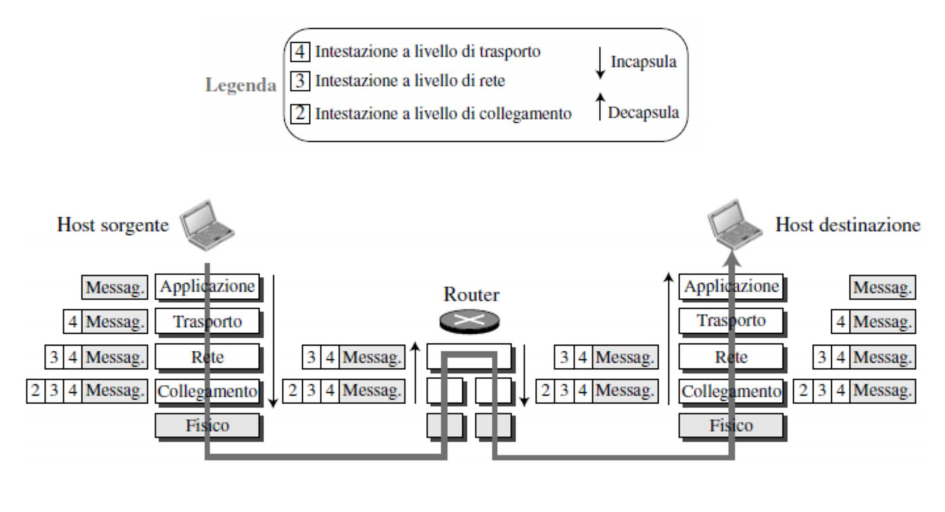
\includegraphics[width=0.9\textwidth]{immagini/Incapsulamento.png}
    \caption*{Incapsulamento}
\end{figure}

\subsubsection{ISO/OSI vs TCP/IP}

\begin{itemize}
    \item ISO/OSI
          \begin{itemize}
              \item generale
              \item definizione di servizio, interfaccia e protocollo
              \item poco efficiente, alcuni livelli poco utili
              \item standard difficili
              \item telco-oriented
              \item poca tempestività
          \end{itemize}
    \item TCP/IP
          \begin{itemize}
              \item standard de facto
              \item implementation driven
              \item specifiche non astratte e rigorose
              \item modello non generale
              \item oltre a TCP/IP, presenza di protocolli minori (per problemi ad-hoc), difficili da rimpiazzare
          \end{itemize}
\end{itemize}

